\section{Payload Design}
\subsection{Mission Objectives}
The mission objective of the MuirSat is to measure the electron temperature and density of the lower ionosphere. Obtaining this data is important for many reasons. The plasma floating potential and temperature are important parameters used in the design of satellites. Furthermore, measuring the ionosphere density will allow orbital decay to be more accurately predicted. Finally, this data will help further research in space weather and will assist in future predictions of space weather.\\

Currently, the plasma properties of the lower ionosphere are not well known due to constraints on maintaining a measurement instrument there for extended periods of time \cite{na_test_2015}. This is because the atmospheric drag is extremely strong in this location and thus it is not economically viable to use a regular satellite to obtain data due to the short orbital life. Currently, the only data available from the ionosphere was obtained from sounding rockets. However, these can only record data for a few minutes at the vertex of their trajectory \cite{na_test_2015}. CubeSats provide a low-cost solution to this problem as they can record data over multiple months with a high spatial resolution. Furthermore, CubeSats can collect data over extended periods of time allowing for the time evolution of the ionosphere to be studied. To fulfil the mission objective, a double Langmuir probe will be used as the payload on the CubeSat. A Langmuir probe can measure plasma properties by inserting multiple conducting probes into a plasma and applying a potential difference between them. For a space based plasma at least two probes are required as there is no reference ground potential.\\

The use of Langmuir probes as a payload on satellites is only a recent occurrence. The QB50 program launched 50 CubeSats into space, 10 of which utilised multi-needle Langmuir probes as the primary payload. The goal of this was to constructed a detailed model of the lower ionosphere. Since the QB50 CubeSats only launched in 2017, there is little feedback on the success of these missions that is publicly available. Regardless of the outcome of this program, further research into the lower ionosphere remains important in understanding the plasma environment for existing satellites. Furthermore, by launching a year after the QB50 program the MuirKat mission will be able to obtain data at a different point during the solar cycle, providing a long-term description of the ionosphere properties. Langmuir probes were also used on NORSAT-1, which is a microsatellite designed by the Norwegian Space Centre. From the initial reports released it appears that the satellite is correctly obtaining data from the ionosphere \cite{university_of_toronto_institute_for_aerospace_studies_space_flight_laboratory_norwegian_2017}. Overall use the of Langmuir probes on satellites is still a novel concept, with early signs indicating success, and there are many more improvements to be made and research to be performed.

\subsection{Theory}
A voltage sweep from a double Langmuir probe produces a current-voltage (abbreviated to IV) curve which has a characteristic shape as shown in Figure \ref{fig:LP_IV_curve}. When a high positive voltage is applied, the current in the plasma consists entirely of electrons and so this is known as the electron saturation region. Conversely, when a large negative voltage is applied the current is composed of positive ions and this is known as the ion saturation region.\\

\begin{figure}[h]
	\centering
	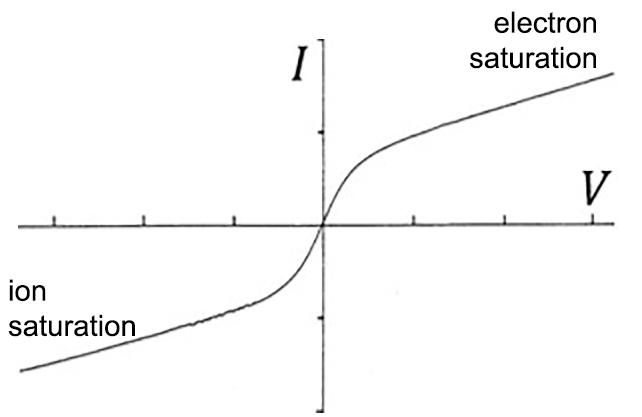
\includegraphics[scale = 0.5]{LP_IV_curve}
	\caption{A typical IV curve for a double Langmuir probe. The electron saturation region exists when the voltage is increased sufficiently high while the ion saturation region exists when the voltage is lowered sufficiently.}
	\label{fig:LP_IV_curve}
\end{figure}

The IV curve contains all of the information required for plasma diagnostics. By analysing the properties of the curve the plasma density and temperature can be computed. The slope of the plot at the origin is given by \cite{naz_development_2014}:

\begin{align} \label{eq:LP_slope}
	\left. \frac{dI}{dV} \right|_{V=0} = \frac{eI_{is}}{2k_B T_e}
\end{align}

where $e$ is the elementary charge and $k_B$ is Boltzmann's constant. $I_{is}$ is the ion saturation current and $T_e$ is the electron temperature. The ion and electron saturation currents are given by the $y$ intercept of the linear fit in their respective regions \cite{tejumola_development_2015}. Lastly the electron density $n_e$ can be computed from:

\begin{align} \label{eq:LP_ne}
	I_{is} = 0.61 n_e e A_p \sqrt{\frac{k_B T_e}{m_i}}
\end{align}

where $A_p$ is the surface area of the probe and $m_i$ is the mass of the ions. These equations allow for the electron temperature and density to be computed by the OBC using the following procedure:

\begin{enumerate}
	\item Perform a least-squares linear fit in the ion saturation region. The $y$ intercept of this is $I_{is}$.
	\item Perform a least-squares linear fit about the origin to determine the slope.
	\item Use $I_{is}$ and equation \eqref{eq:LP_slope} to compute $T_e$.
	\item Use equation \eqref{eq:LP_ne} to compute $n_e$.
\end{enumerate}

This procedure was implemented in the OBC code and is given in Appendix  \ref{app:code_payload}. In order to improve the accuracy of the results, multiple samples were taken at each voltage value and were averaged. This reduces the impact of noise upon the results. It was found that 100 samples at each voltage was sufficient to minimize the fluctuations in the recorded data.

\subsection{Circuit Design}
An overview of the circuit that was designed for the Langmuir probe is given in Figure \ref{fig:LP_circuit_diagram}. A voltage booster takes 5V from the bus and steps it up to 24 V. A capacitor is placed across the input of the booster in order to provide a smooth input in the event of voltage fluctuations. The stepped up voltage is then fed into the MAX14870 Motor Controller. This is able to sweep a voltage from zero to the input value, as well as reverse the polarity. This board is controlled by three digital pins which; enable the output, control the polarity, and change the magnitude of the output. As the motor controller outputs a PWM signal, it is smoothed by an RC filter across the outputs.\\

\begin{figure}[h]
	\centering
	\includegraphics[width=\textwidth]{LP_circuit_diagram}
	\caption{Complete circuit for the Langmuir probe.}
	\label{fig:LP_circuit_diagram}
\end{figure}

The signal is then passed to the probes. Following the probes is a voltage rectifier constructed from four diodes. This is so the current sensor receives a positive polarity regardless of the polarity given to the probes. Finally the low current sensor is connected to the output of the voltage rectifier. To measure the current, two operational amplifiers are employed. The OPA277P is a high precision amplifier that is used to amplify the current by a factor given by the gain resistor. The MCP601P is a normal operational amplifier that is used to correct for the current drop that is caused by the act of measuring. In order for this to function correctly, it requires a separate power source which is floating relative to the input power. To achieve this, a coin cell battery has been used on the circuit. For the complete CubeSat, a floating power source will be constructed using the on board power, however this circuitry is too complex for the prototype and has been omitted.

\subsection{Sensing Accuracy}
In this section some of the properties of the Langmuir probe instrument are calculated and described. The current gain factor was chosen to be $620,000$. The maximum value the voltage can be amplified to is that of the battery, in this case it is 3V. This means that the sensor will saturate when attempting to measure a current of 4.8$\mu$A or greater. Given that the expected collected current will be in the range of $3.7\times 10^{-7}$ to $3.7\times 10^{-6}$ A \cite{na_test_2015}, the chosen gain factor is quite suitable.\\

The Teensy has a resolution of 10 bits for the analogue input pins. Dividing the current range from zero to 4.8$\mu$A into 10 bits results in a reading resolution of $0.0047\mu$A steps. This places a limit on the precision of a single current measurement as $\pm 0.00235\mu$A. In contrast, the PWM output only has a resolution of 8 bits. For a negative to positive voltage sweep, this results in 511 data points collected.\\

Lastly, an ammeter was placed on the 5V input to the circuit in order to measure the net current draw. The voltage output was set to the maximum value and the current draw from the power supply was measured to be 2.1 mA. This means that running the Langmuir probe consumes 10 mW of power. The current and power draw is extremely low due to the low currents being measured.

\subsection{Ohmic Resistor Validation}
To validate the Langmuir probes, an ohmic resistor was placed between the probes and a sweep was performed. The resistance of the resistor was measured to be $R=3.98$ M$\Omega$ with an multimeter. The results are shown in Figure \ref{fig:LP_plot_ohmic}. It should be noted that when zero voltage is applied there is still a current measured which has magnitude $1.24$ $\mu$A. This is background thermal noise. In order to verify that this is indeed the thermal noise, the result will be compared to the analytic result, given by Johnson-Nyquist noise formula:

\begin{align*}
	V_n = \sqrt{4k_B TR \Delta f}
\end{align*}

for a temperature of $T=298$ K, resistance of $R=3.98$ M$\Omega$ and bandwidth of $\Delta f =16$ Hz the thermal noise is computed to be $V_n =1.02$ $\mu$V. This is close to the value observed from the experiment, thus verifying that this offset is thermal noise. Interestingly, it should be noted that this offset is asymmetric as it is far smaller in magnitude when a negative polarity is applied. It is not understood why this is the case as the voltage rectifier ensures the current sensor always receives a positive current to measure. One possibility is that when the polarity is reversed, the current sensor is now measuring the noise upstream of the resistor which possible has less impact than when measuring downstream of the resistor. To counteract the thermal noise the OBC will sample the current with no voltage applied and record this value as the offset. The sweep is then performed and this offset is subtracted, producing the correct plot.\\

\begin{figure}[h]
	\centering
	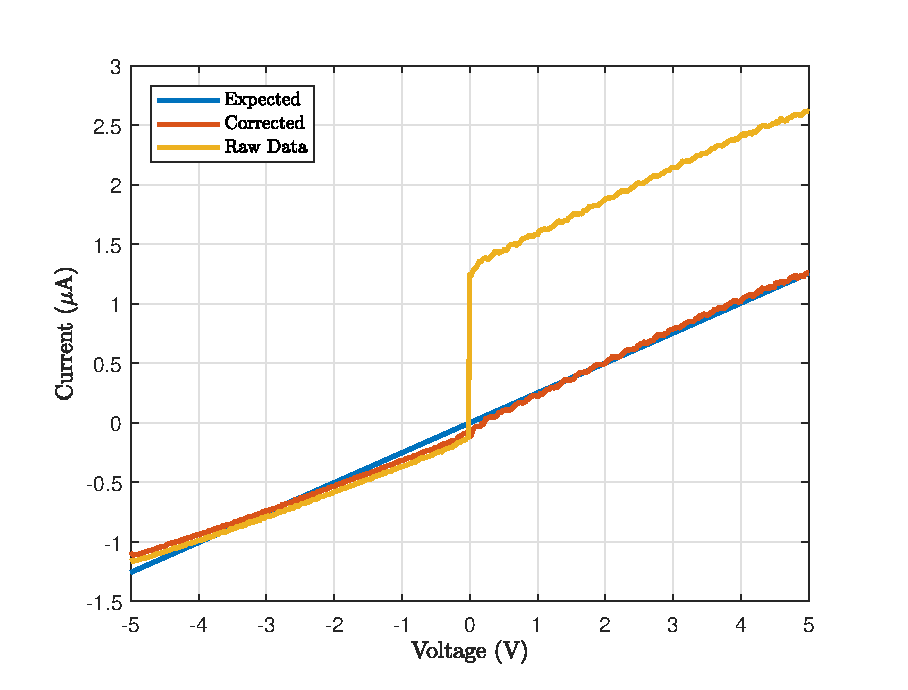
\includegraphics[width=\textwidth]{LP_plot_ohmic}
	\caption{The IV curve generated when a 3.98 M$\Omega$ resistor was placed across the probes. From the slope of the plot, the resistance is calculated to be $4.02$ M$\Omega$.}
	\label{fig:LP_plot_ohmic}
\end{figure}

It can be seen that there are small ripples in the current, which is a consequence of the smoothed PWM signal that was applied to the probes. By increasing the number of samples taken at each voltage value the magnitude of this ripple can be reduced. Lastly, the resistance is the inverse of the slope of this line, which was measured to be 4.02 M$\Omega$. This value is quite close to the measured value, which validates the ability of the circuitry to accurately measure current of the order $\mu$A.

\subsection{Further Testing}
As the capability to accurately measure micro amp current has been verified, the final testing required is a plasma environment test. The Langmuir probe will be connected to a micro-controller in a self contained system that is placed in a vacuum environment. A plasma will be established and multiple voltage sweeps will be performed and the data will be recorded. This data will be used to verify that the probes can obtain a correct IV curve. Furthermore, obtaining experimental data will allow for the data processing algorithm to be tested and validated. Once the data is obtained the algorithm can be refined, completing the design of the Langmuir probe.

\subsection{Probe Deployment Mechanism}
Two probes are required for the mission, where a single probe is a thin conducting metal rod that is extruded from the CubeSat into the plasma. For the real CubeSat, a thin rod of diameter 2 mm and length 60 mm is suitable for this purpose. However, as this will be need to be custom made, an `off the shelf' replacement will be used for the prototype in the form of a sewing needle. The probes are not required to point in any direction in order to function properly as the plasma is locally isotropic. The probes are constructed from stainless steel since the melting point is higher than the temperature of the ionosphere plasma. The probes are initially internal to the CubeSat, during launch and when the CubeSat is deployed. A mechanism has been designed which allows for the two probes to be extruded upon command. To assess possible solutions to this problem a trade off table (Table \ref{table:trade}) was used.\\

\begin{table}[]
\centering
\begin{tabular}{@{}lcccc@{}}
\toprule
                            & \textbf{Rack and Pinion} & \textbf{Bevel Gears} & \textbf{Spur Gears} & \textbf{Torsion Springs} \\ \midrule
Ease of Manufacture         & 3                               & 1                             & 4                          & 5                        \\
Reliability and Reusability & 5                               & 2                             & 4                          & 1                        \\
Weight and Size             & 1                               & 3                             & 3                          & 3                        \\
Displacement Allowed        & 5                               & 4                             & 4                          & 4                        \\
Electronic Requirements     & 1                               & 3                             & 3                          & 3                        \\
\textbf{Total}              & \textbf{15}                     & \textbf{13}                   & \textbf{18}                & \textbf{16}              \\ \bottomrule
\end{tabular}
\caption{Trade off table comparing proposed payload mechanisms}
\label{table:trade}
\end{table} 

The bevel gear system is clearly the worst design, using a central gear to rotate two smaller pinions that rotates the probes from a horizontal to vertical position along the $-z$ face of the MuirKat. Its issues stem from difficulties with manufacturing and design. The payload assembly was to be 3D printed using ABS and helical bevel gears were outside the scope of the capabilities of any printer available for this project, thus this design was rejected. The linear rack and pinion system was the only design to incorporate redundancy, involving two racks and two pinion gears that moved the probes linearly out along the $x$ direction through the use of a servo. However, since the Langmuir probes must come in pairs, even if one servo were to fail it makes no sense to deploy just one probe. Thus, despite containing mechanical redundancy, the unique requirements of the payload mean true redundancy would require four servo motors. This is reflected in the poor size/weight and electronic scores, leading to the rejection of this design. Lastly, rotary spur gears were selected over torsion springs, since the spur gears have comparable performance in all areas but are able to be used multiple times. The final payload assembly is shown in Figure \ref{fig:payload}. Note that that the torsion spring system still required electronics to operate in the form of a fuse wire that would be melted to release the spring energy and deploy the probes. In addition, although it is not listed in the table, the gear assemblies all perform better under vibration than the spring assembly since they don't have a natural tendency to displace under oscillation.\\

\begin{figure}[!h]
\centering 
\includegraphics[width=0.5\textwidth]{payload.JPG}
\caption{Computer render of the final payload assembly to be manufactured using 3D printed ABS (FDM process courtesy of Quang Vuong, chief of CS Sydney Solar)}
\label{fig:payload}
\end{figure}

The mechanism utilises a 50mm diameter spur gear at the centre, actuated by a sub-micro servo motor. The servo receives power from the battery and data from the OBC. Upon turning, two half-size (25 mm diameter) pinion gears are meshed at a 20$^{\circ}$ pressure angle. This rotation is put to work when the Langmuir probes are mounted on top. The probes `fan' out at 90$^{\circ}$ to the side of the MuirKat, anti-parallel to each other. This mechanism was the ideal solution for the MuirKat, meeting all the design requirements of the structural and payload subsystems whilst consuming little power and being simple to program.\\ 

In addition to housing the payload assembly, a secondary plate was added to make better use of the $z$ space occupied by the servo. Rather than waste this vertical distance, the second plate allows for the winding of the $z$ magnetorquer, cleaning up the satellite's assembly in the process.
